\section{Charm's Architecture}
\label{sec:arch}

The goal of Charm is to decode weak transmissions, which could not be decoded
by any individual gateway, by collating receptions from multiple gateways at
the cloud. At one level, this  enables us to expand network coverage area
reaching clients deep inside buildings, underground or in outer reaches of the
city. More fundamentally, it saves energy on the vast majority of client
devices, even if they are within range of some gateways by allowing them to
increase their data rate without experiencing any loss in performance. Our
results in Sec.~\ref{sec:energy-savings} demonstrate that lowering transmit
time results in a direct and significant impact on battery life.

Fig.~\ref{fig:architecture} depicts Charm's architecture where we assume the
gateways can be user-deployed  both indoors and outdoors, at a cost of a few
hundred dollars. These base stations have an Ethernet backhaul to the cloud
that accommodate a maximum uplink bandwidth of a few megabits per seconds.
Much like the standard LoRaWAN architecture, MAC-layer scheduling is performed
at the cloud with gateways relaying their received data to the cloud. However,
to accommodate decoding weak received signals, we also allow gateways to ship
raw received I/Q signals from feeble low-power clients to the cloud. The cloud
aggregates such weak signals and coherently combines them to decode the
underlying data bits from feeble receptions across multiple gateways. In other
words, Charm performs a joint optimization of the  PHY-layer at the cloud,
simultaneously improving battery life and range of low-power clients at the
expense of increased computation at the cloud.

Realizing a scalable and real-time system based on the above architecture
is challenging both at the gateways and the cloud:
\begin{itemize}
\item {\bf At the Gateway: } Given that signals from weak LPWAN
clients are often well below the noise floor, gateways are unaware of these
packets in the received signal. This means that base stations must effectively
send all their received raw signal data to the cloud to detect and decode weak
signals, stressing their limited uplink bandwidth.
\item {\bf At the Cloud: } The cloud must identify signals from which
gateways need to be combined to recover transmitted data from multiple
clients. At city-scale, it is conceivable that overlapping weak transmissions
from different clients are received at the same time by gateways, making data
recovery challenging at the cloud. Additionally due to the use of low-cost
hardware that lacks precise time synchronization, each of the gateways adds
clock and frequency errors to the captured signals. These must be resolved
before the signals can be combined.
\end{itemize}

\begin{figure}[!htb]
    \centering
    \compactimg
    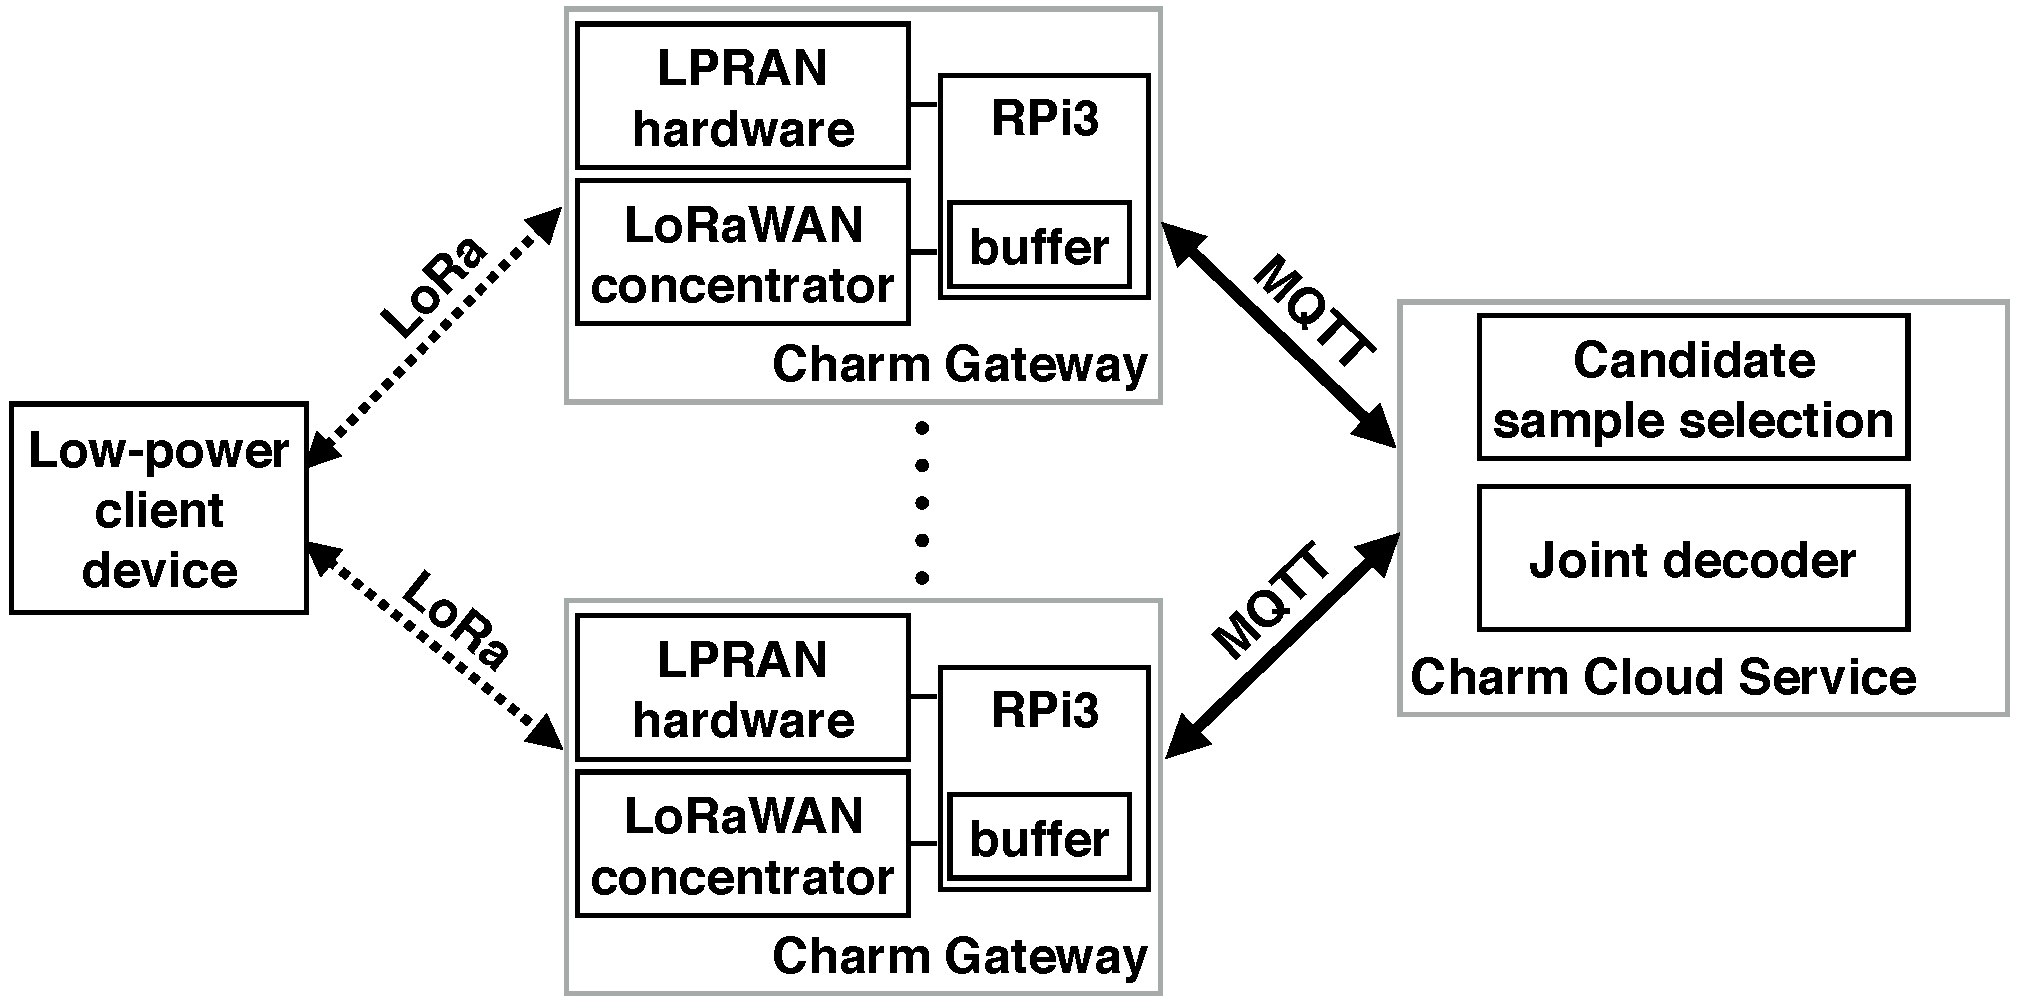
\includegraphics[width=0.45\textwidth]{figures/charm-architecture_cropped.pdf}
    \compactimg
    \caption{Architecture of Charm}
    \label{fig:architecture}
    \compactimg
\end{figure}

The rest of this paper describes Charm's solutions to each of these
challenges. Specifically, Charm makes two key contributions: (1) A software
interface at the gateway to identify weak transmissions to ship to the cloud,
and a hardware design that facilitates these decisions in real-time; (2) A
scalable cloud based PHY-layer processing system at the cloud that can operate
at city-scale. Next we elaborate on each of these components.